\section{Mathématiques}

%-----------------------
\subsection{Écrire des Mathématiques}

\begin{frame}[fragile]{L'environnement mathématique}
  \framesubtitle{Inclure des formules dans le texte}
  \begin{itemize}
      \item On peut ouvrir un environnement mathématique entre deux symboles \textbf{\$}.

  \begin{center}
    \begin{tabular}{lll}
      \lstinline|$x + 1 = 2$| & $x + 1 = 2$\\
      \medskip
      \lstinline|$\frac{1}{x}$| & $\frac{1}{x}$\\
    \end{tabular}
  \end{center}
      \item Les opérateurs et symboles, comme les autres commandes, commencent par \textbf{\textbackslash}, sauf \lstinline|+, -, /, ^,| et \lstinline|_|
      \begin{center}
          \begin{tabular}{llr}
              \lstinline|$a^{11}$| & $a^{11}$ & Good \\
              \lstinline|$a^11$| & $a^11$ & Bad ! \\
              \lstinline|$\sin(x)$| & $\sin(x)$ & Good \\
              \lstinline|$sin(x)$| & $sin(x)$ & Bad !\\
              \lstinline|$\frac{\Theta}{\sqrt{\beta}}$| & $\frac{\Theta}{\sqrt{\beta}}$ & Very good !
          \end{tabular}
      \end{center}
      \item Les packages \lstinline|amsmath| et \lstinline|amssymb| apportent beaucoup d'environements et symboles supplémentaires très utiles, à inclure par défaut.
  \end{itemize}
\end{frame}

\begin{frame}[fragile]{L'environnement mathématique}
  \framesubtitle{Inclure des formules centrées hors du texte}
  \begin{itemize}
  \item On peut aussi ajouter une formule mathématique centrée hors du texte entre \lstinline|\[ ... \]|.
  \vspace{0.5cm}
  \begin{columns}
    \begin{column}{0.45\textwidth}
      \begin{lstlisting}[style = nonumbers]
  L'expression $\sin(x)$ peut s'écrire de différents manières. En effet, il a été démontré que

  \[
    \sin(x) =
    \frac{e^{iz} - e^{-iz}}{2i}
  \]

  avec $i$ étant l'unité imaginaire.
      \end{lstlisting}
    \end{column}
    \begin{column}{0.45\textwidth}
      L'expression $\sin(x)$ peut s'écrire de différents manières. En effet, il a été démontré que

      \[ \sin(x) = \frac{e^{iz} - e^{-iz}}{2i} \]

      avec $i$ étant l'unité imaginaire.
    \end{column}
  \end{columns}
  \end{itemize}
\end{frame}

%-----------------------
\subsection{Les Matrices}

\begin{frame}[fragile]{Matrices}
  \begin{itemize}
    \item Les matrices s'écrivent avec l'environnement \lstinline|matrix| (fonctionnement semblable à \lstinline|tabular|).
      \begin{columns}
        \begin{column}{0.45\textwidth}
          \begin{lstlisting}[style=nonumbers]
\[
  \begin{matrix}
    \alpha & \beta \\
    \gamma & \delta \\
  \end{matrix}
\]
          \end{lstlisting}
        \end{column}
        \begin{column}{0.45\textwidth}
          \[\begin{matrix}
            \alpha & \beta \\
            \gamma & \delta \\
            \end{matrix}\]
        \end{column}
      \end{columns}
    \item On ajoute des délimiteurs avec \lstinline|pmatrix|,\lstinline|vmatrix|,\ldots{}
      \begin{columns}
        \begin{column}{0.45\textwidth}
          \begin{lstlisting}[style=nonumbers]
\[
  \begin{pmatrix}
    a + b & c \\
    d & e + f \\
  \end{pmatrix}
\]
          \end{lstlisting}
        \end{column}
        \begin{column}{0.45\textwidth}
          \[\begin{pmatrix}
            a + b & c \\
            d & e + f \\
            \end{pmatrix}\]
        \end{column}
      \end{columns}
    \item Les différents délimiteurs sont
      \begin{center}
        \begin{tabular}{llllll}
            \lstinline|bmatrix| & [ ] & \lstinline|Bmatrix| & \{ \} & \lstinline|pmatrix| & ( ) \\
            \lstinline|vmatrix| & | | &	\lstinline|Vmatrix| & || ||
        \end{tabular}
      \end{center}
  \end{itemize}
\end{frame}

\begin{frame}[fragile]
  \frametitle{Les délimiteurs}
  \begin{itemize}
      \item Par défaut \LaTeX utilise des parenthèses de taille standard, ne s'adaptant pas au contenu qu'elles contiennent.
      \begin{lstlisting}[style=nonumbers]
\[ ( \frac{x^2}{y^3} ) \]
\end{lstlisting}
\[ (\frac{x^2}{y^3}) \]
      \item La solution ? Les commandes \lstinline|\left...| et \lstinline|\right...| permettent d'adapter automatiquement la taille des parenthèses.
      \begin{lstlisting}[style=nonumbers]
\[ \left( \frac{x^2}{y^3} \right) \]
\end{lstlisting}
\[ \left( \frac{x^2}{y^3} \right) \]
      \item Fonctionne aussi avec \lstinline|\left\{ \right\}| ou \lstinline|\left[ \right]|
\[ \left\{\frac{x^2}{y^3}\right\} \qquad \left[\frac{x^2}{y^3}\right] \]
  \end{itemize}
\end{frame}

%-----------------------
\subsection{Formules Numérotées}

\begin{frame}[fragile,allowframebreaks]{Formules Numérotées}
  \begin{itemize}
    \item L'environnement \lstinline|equation| permet d'écrire des équations numérotées.
    \begin{columns}
      \begin{column}{0.5\textwidth}
        \begin{lstlisting}[style=nonumbers]
\begin{equation}
    c^2 = a^2 + b^2
\end{equation}
        \end{lstlisting}
      \end{column}
      \begin{column}{0.5\textwidth}
        \begin{equation}
                c^2 = a^2 + b^2
        \end{equation}
      \end{column}
    \end{columns}

    \item L'environnement \lstinline|align| permet d'écrire des équations alignées et numérotées. \lstinline|align*| aligne plusieurs équations sans les numéroter.
    \item On peut ne pas numéroter une équation en plaçant \lstinline|\nonumber| à la fin de la ligne.
      \begin{columns}
        \begin{column}{0.5\textwidth}
          \begin{lstlisting}[style = nonumbers]
I like trains and the equations
\begin{align}
e^{i\pi} + 1 & = 0\\
f(t) & = A\cos(\omega t + \phi) \nonumber
\end{align}
I also know that
\begin{align*}
1 + 1 & = 2\\
2 + 3 & = 5
\end{align*}
          \end{lstlisting}
        \end{column}
        \begin{column}{0.5\textwidth}
          I like trains and the equations
          \begin{align}
e^{i\pi} + 1 & = 0\\
f(t) & = A\cos(\omega t + \phi) \nonumber
          \end{align}
          I also know that
          \begin{align*}
1 + 1 & = 2\\
2 + 3 & = 5
          \end{align*}
        \end{column}
      \end{columns}
\framebreak
    \item Utilisation de l'environnement \lstinline|aligned| pour faire un système d'équation (utilisation semblable à \lstinline|align|).
    \begin{columns}
      \begin{column}{0.5\textwidth}
        \begin{lstlisting}[style=nonumbers]
  \[
      \left\{
          \begin{aligned}
           x^2 + y &= 3 \\
           \frac{y}{x} &= 0.42
          \end{aligned}
      \right.
  \]
        \end{lstlisting}
      \end{column}
      \begin{column}{0.5\textwidth}
            \[ \left\{\begin{aligned}
                x^2 + y &= 3 \\
                \frac{y}{x} &= 0.42
            \end{aligned}\right. \]
      \end{column}
    \end{columns}
  \end{itemize}
\end{frame}

%-----------------------
\subsection{Les maths et les polices}

\begin{frame}[fragile]{Les maths et les polices}
  \begin{itemize}
    \item Parfois, certaines variables sont composées de plusieurs lettres. On doit utiliser des polices différentes comme \lstinline|\mathrm| ou \lstinline|\mathsf|. \lstinline|\mathcal| produit des lettres \og calligraphiques \fg{}.
      \begin{center}
        \begin{tabular}{lll}
                  \lstinline|$Var(x)$| & $Var(x)$ & Bad ! \\
                  \lstinline|$\mathrm{Var}(x)$| & $\mathrm{Var}(x)$ & Good \\
                  \lstinline|$F_{machine}$| & $F_{machine}$ & Bad ! \\
                  \lstinline|$F_\mathrm{machine}$| & $F_\mathrm{machine}$ & Good \\
                  \lstinline|$\mathcal{M}$| & $\mathcal{M}$ &
        \end{tabular}
      \end{center}
    \item Les ensembles s'écrivent à l'aide de la police \lstinline|\mathbb|.
      \begin{center}
          \begin{tabular}{cccc}
          \lstinline|$\mathbb{N}$| & $\mathbb{N}$ & \lstinline|$\mathbb{Z}$| & $\mathbb{Z}$ \\
          \lstinline|$\mathbb{D}$| & $\mathbb{D}$ & \lstinline|$\mathbb{Q}$| & $\mathbb{Q}$ \\
          \lstinline|$\mathbb{N}$| & $\mathbb{R}$ & \lstinline|$\mathbb{C}$| & $\mathbb{C}$
          \end{tabular}
      \end{center}
  \end{itemize}
\end{frame}

%-----------------------
\subsection{Large Operators}

\begin{frame}[fragile]{Large Operators}
  \begin{itemize}
    \item Voici quelques opérateurs utiles:
      \begin{center}
          \begin{tabular}{lll}
          \lstinline|\min_{x \in \mathbb{R}}| & $\min_{x \in \mathbb{R}}$ & $\displaystyle\min_{x \in \mathbb{R}}$ \\
          \lstinline|\max_{x \in \mathbb{R}}| & $\max_{x \in \mathbb{R}}$ & $\displaystyle\max_{x \in \mathbb{R}}$ \\
          \lstinline|\lim_{x \to \infty}| & $\lim_{x \to \infty}$ & $\displaystyle\lim_{x \to \infty}$ \\
          \lstinline|\sum_{i=1}^n| & $\sum_{i=1}^n$ & $\displaystyle\sum_{i=1}^n$ \\
          \lstinline|\prod_{i=1}^n| & $\prod_{i=1}^n$ & $\displaystyle\prod_{i=1}^n$
          \end{tabular}
      \end{center}
    \item Le résultat ne sera pas le même qu'on soit dans un texte ou dans une équation.
    \item Une liste des opérateurs mathématiques les plus courant est disponible à cette adresse : \url{http://www.univ-irem.fr/lexique/res/Annexe_E_-_Liste_des_symboles_mathematiques_usuels__LaTeX_.pdf}
  \end{itemize}
\end{frame}

\begin{comment}
\subsection{Définir des commandes}
%TODO : Exemple plus simple et \operatorname{}
\begin{frame}[fragile]{Définition de commandes, plus d'excuse !}

\begin{itemize}
    \item Définition de nouvelles commandes par \lstinline|\newcommand{nom}{définition}|
    \item Dans un environnement mathématique, on utilise \lstinline|\DeclareMathOperator{nom}{définition}|

    \begin{lstlisting}[style=nonumbers]
\DeclareMathOperator{\sumN}{\sum_{i=1}^n}

\DeclareMathOperator{\var}{\mathrm{Var}}
    \end{lstlisting}

    \begin{columns}
        \begin{column}{0.5\textwidth}
          \[\var(x) = \pi\]
            \[\sumN \frac{i}{i+1}\]
        \end{column}
        \begin{column}{0.5\textwidth}
            \begin{lstlisting}[style=nonumbers]
\[ \var(x) = \pi \]
\[ \sumN \frac{i}{i+1} \]
            \end{lstlisting}
        \end{column}
    \end{columns}

\end{itemize}
\end{frame}

\begin{frame}[fragile]{L'environnement mathématique}
\framesubtitle{Forcer un espacement}
Rarement utile !

\begin{center}
  \begin{tabular}{ll}
    Commande & espacements en mu (espace normal${}={}$6mu)\\
    \hline
    \lstinline|\!|     & $-$3\\
    \lstinline|\,|     &  3\\
    \lstinline|\:|     &  4\\
    \lstinline|\;|     &  5\\
    \lstinline|\ |     &  6\\
    \lstinline|\quad|  & 18\\
    \lstinline|\qquad| & 36
  \end{tabular}
\end{center}
\end{frame}

\begin{frame}[fragile]{L'environnement mathématique}
\framesubtitle{Forcer un espacement : Exemples}
\begin{columns}
  \begin{column}{0.5\textwidth}
    \begin{lstlisting}
\begin{align*}
  a & = u + v + w + x + y\\
    & \quad + z
\end{align*}
    \end{lstlisting}
  \end{column}
  \begin{column}{0.5\textwidth}
\begin{align*}
  a & = u + v + w + x + y\\
    & \quad + z
\end{align*}
  \end{column}
\end{columns}

Erreur courante: les ensembles ont besoin d'espacement (i.e. \lstinline|\,|) en compréhension mais pas en extension.
\begin{columns}
  \begin{column}{0.5\textwidth}
    \begin{lstlisting}
\begin{align*}
  \mathbb{R}_+ & = \{\, x \in \mathbb{R} \mid R \geq 0 \,\}\\
  \mathbb{R}_+ & = \{\, x \in \mathbb{R} : R \geq 0 \,\}\\
  \mathbb{N} & = \{0, 1, 2, 3, 4, \ldots\}\\
\end{align*}
    \end{lstlisting}
  \end{column}
  \begin{column}{0.5\textwidth}
\begin{align*}
  \mathbb{R}_+ & = \{\, x \in \mathbb{R} \mid R \geq 0 \,\}\\
  \mathbb{R}_+ & = \{\, x \in \mathbb{R} : R \geq 0 \,\}\\
  \mathbb{N} & = \{0, 1, 2, 3, 4, \ldots\}\\
\end{align*}
  \end{column}
\end{columns}
\end{frame}
\end{comment}

%-----------------------
\subsection{La physique}

\begin{frame}[fragile]
  \frametitle{Les unités}
  \begin{itemize}
    \item Le package \lstinline|\usepackage{siunitx}| permet de gérer l'utilisation d'unités dans vos formules.
        \begin{center}
          \begin{tabular}{ll}
            \num{314e-2} & \lstinline|\num{314e-2}|\\
            \ang{42} & \lstinline|\ang{42}|\\
            \si{g_{polymer}~mol_{cat}.s^{-1}} &
            \lstinline|\si{g_{polymer}~mol_{cat}.s^{-1}}|\\
            \si{\square\volt\cubic\lumen\per\farad} &
            \lstinline|\si{\square\volt\cubic\lumen\per\farad}|\\
            \SI{5e-6}{\meter\per\second\per\ohm} &
            \lstinline|\SI{5e-6}{\meter\per\second\per\ohm}|\\
            \SI[per-mode=symbol]{5.3e9}{\meter\per\second} &
            \lstinline|\SI[per-mode=symbol]{5.3e9}{\meter\per\second}|\\
            \SI[per-mode=symbol]{5.3e9}{\meter\per\second\per\ohm} &
            \lstinline|\SI[per-mode=symbol]{5.3e9}{\meter\per\second\per\ohm}|\\
            \SI[per-mode=fraction]{5e6}{\joule\per\second} &
            \lstinline|\SI[per-mode=fraction]{5e6}{\joule\per\second}|\\
            \SI{-273.15}{\celsius} &
            \lstinline|\SI{-273.15}{\celsius}|
          \end{tabular}
        \end{center}
    \item Super doc sur \url{http://ctan.org/pkg/siunitx}
  \end{itemize}
\end{frame}

\begin{frame}[fragile]
  \frametitle{Quatrième exercice}
  \begin{center}
      \fbox{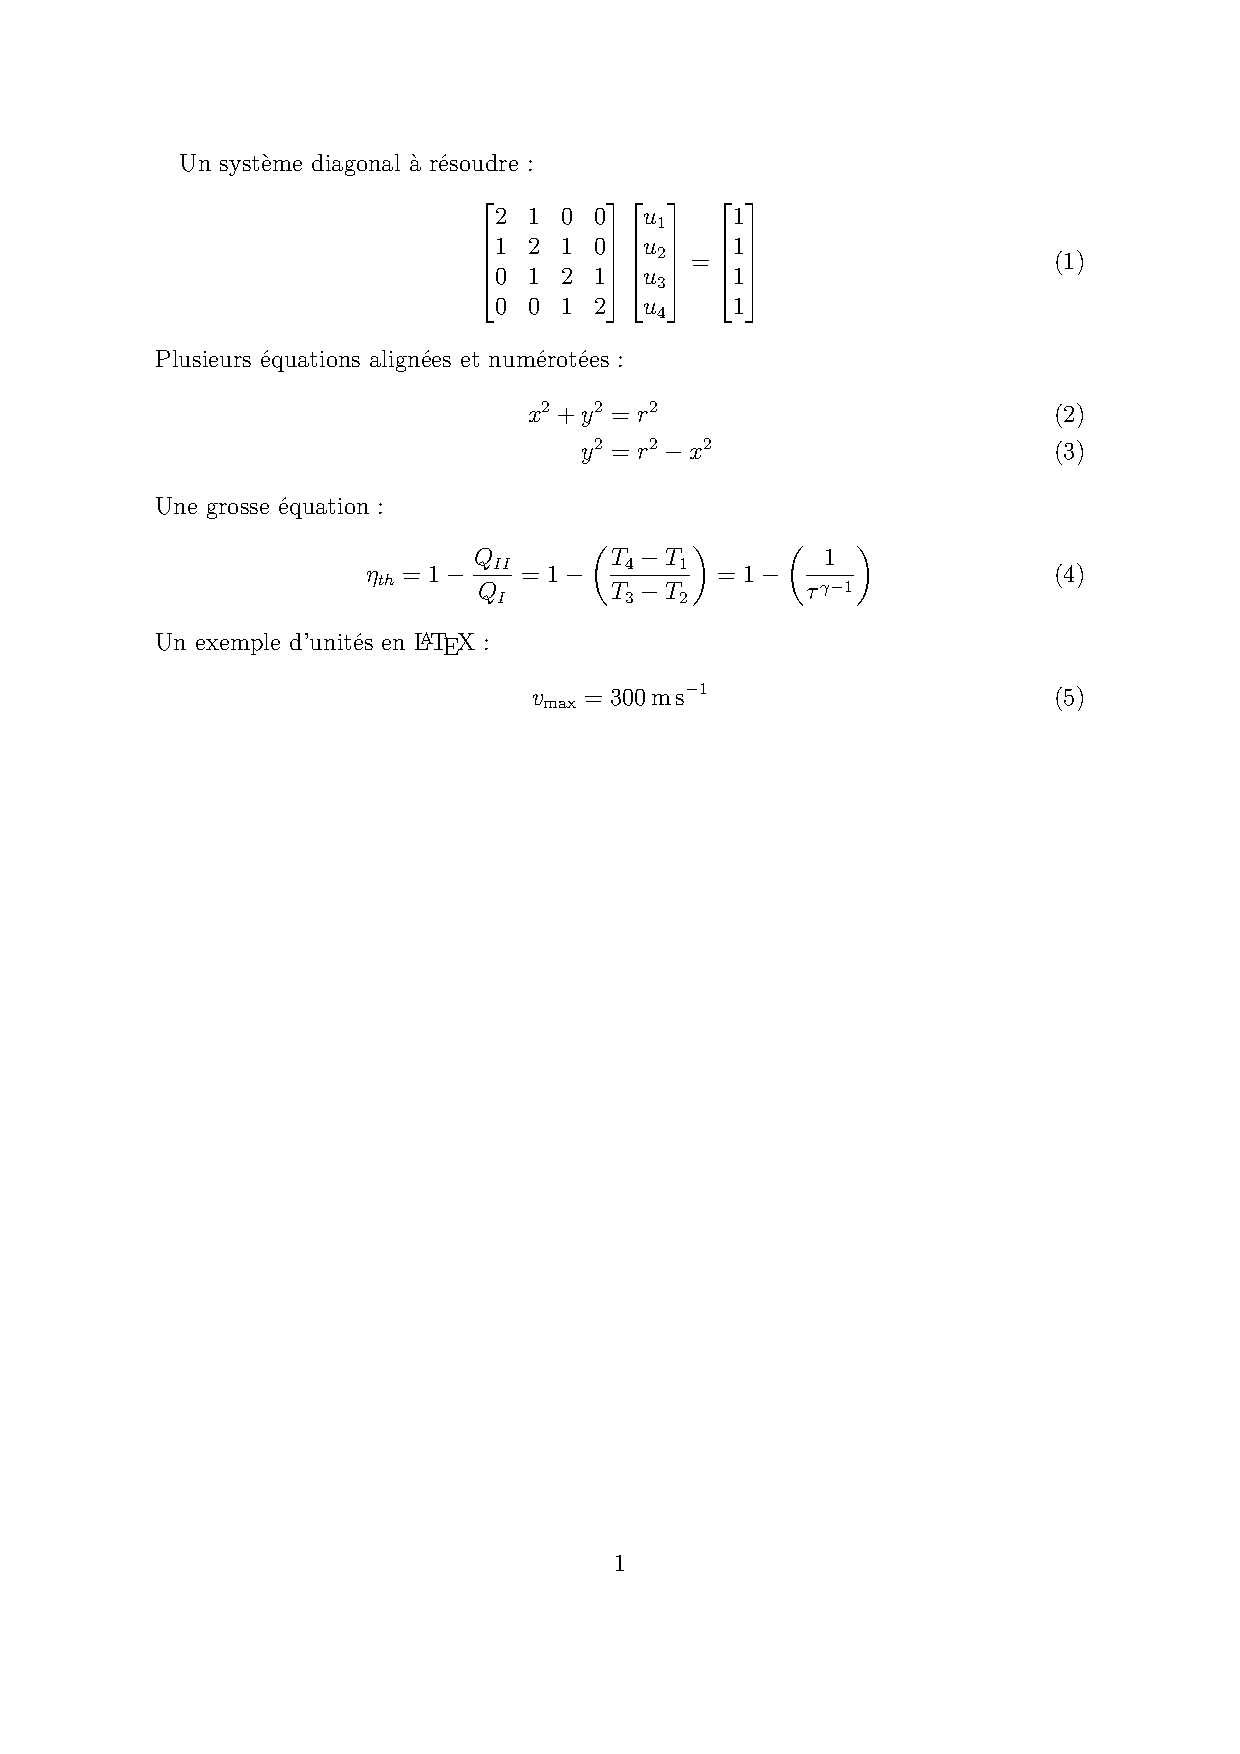
\includegraphics[width=0.8\textwidth,trim={2cm 16cm 2cm 2cm},clip]{../build_latex/exercices/3/main.pdf}}
  \end{center}
\end{frame}

\begin{frame}[fragile]{Quatrième exercice (solution)}
  \begin{center}
  Lien Overleaf de la solution du quatrième exercice \url{https://www.overleaf.com/read/dqdzcnzsmnsh}
  \end{center}
\end{frame}
